%&latex

\documentclass[conference]{IEEEtran}
\usepackage[cmex10]{amsmath}
\usepackage{algorithmic}
\usepackage{array}
\usepackage{eqparbox}
\usepackage[english]{babel}
% *** SUBFIGURE PACKAGES ***


\usepackage{graphicx}
\usepackage{epsfig}
\usepackage{epstopdf}
\usepackage{amsmath} 
%\usepackage[caption=false]{caption}
\usepackage[font=footnotesize]{subfig}
\usepackage{stfloats}
\usepackage{float}
\usepackage{subfig}
\usepackage{amssymb}
\usepackage{cite} 
\usepackage[T1]{fontenc}
%\usepackage{hyperref}
\begin{document}

\title{Proyecto de Investigación de cotizador automático por medio de ChatBots}
\author
{
\IEEEauthorblockN{D.~Figueroa-Castañeda}\\
\IEEEauthorblockA
{
	Universidad Interamericana~ Maestría en automatización industrial, \\manufactura 		digital, y robótica\\
	Puebla,~Mexico \\
	email: \{d.figueroa@lainter.edu.mx}
}



% The paper headers
\markboth{}%
{Shell \MakeLowercase{\textit{et al.}}: Bare Demo of IEEEtran.cls for Journals}

% make the title area
\maketitle


 
\begin{abstract}
 ~En ésta investigación se abordará la integración de programas con capacidad de interactuar por medio de texto con usuarios humanos, conocidos como ChatBot's, para la automatización del proceso de cotización de productos y servicios a través de Internet, en específico, del servicio de Impresión 3D y manufactura aditiva. A través de la creación de un ChatBot para interacuar en Telegram y Facebook desarrollado en Node-RED, una plataforma de programación visual que permite integrar diferentes servicios WEB a través de API's y control de Hardware facilmente, permitiendo administrar también el flujo de trabajo de una granja de impresoras 3D.
\end{abstract}
\vspace{0.5cm}
\textbf{Keywords}:  ChatBot, Node-RED, Cotizador automático, Impresión 3D.

\IEEEpeerreviewmaketitle
\section{Introduccion}
\IEEEPARstart{I}n recent decades,... This paper is organized as follows. In Section $\mathbf{II}$, ... In Section $\mathbf{IV}$... Some simulations in Section $\mathbf{VI}$. Finally, the conclusions are presented in Section $\mathbf{VII}$.

\section{Homotopic Continuation Method}

Homotopy continuation method..

\begin{equation}
\label{ohm}
V=I*R:\quad\mathbb{R}^{n}\longrightarrow\mathbb{R}^{n},
\end{equation}

The system:  
 \begin{equation}
    \label{Homotopia_G}
     H(x,\lambda)= \lambda f(x)+ (1-\lambda)(f(x)- f(x_0))=0,
 \end{equation}
 
 \begin{figure}
 	
\includegraphics[scale=1]{imagenes/img1.eps}
 	\caption{Imagen de prueba}
 	\label{fig:img1}
 \end{figure}
     
     
     
 where,   $\lambda$ is the homotopy parameter,  $x_0$  is the starting point, $H( x,\lambda) :\mathbb{R}^{n+1}\longrightarrow \mathbb{R}^{n} \text{,} \quad{x} \in\mathbb{R}^{n}$. 
\section{Obstacles}
HPPM uses the...%-----------------------------------------------------------------------------------------------------------

\section{Spherical}
 \begin{figure}[H]
\begin{center}
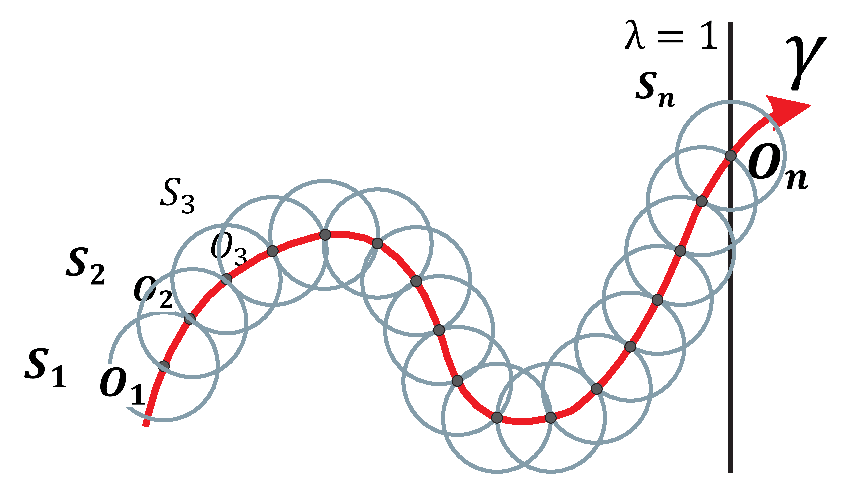
\includegraphics[width=0.2\textwidth]{imagenes/hiper2.eps} 
\caption{ Seguimiento.}
\label{fig:hiper2}
\end{center}
\end{figure}    


  \begin{figure}[H]
\begin{center}
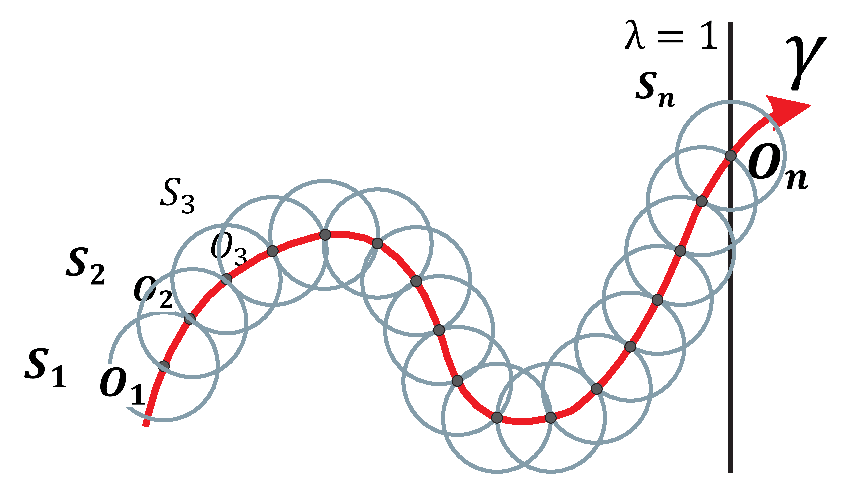
\includegraphics[width=0.2\textwidth]{imagenes/hiper2.eps} 
\caption{ Seguimiento.}
\label{fig:hiper3}
\end{center}
\end{figure}    
  
\begin{figure}[H]
\begin{center}
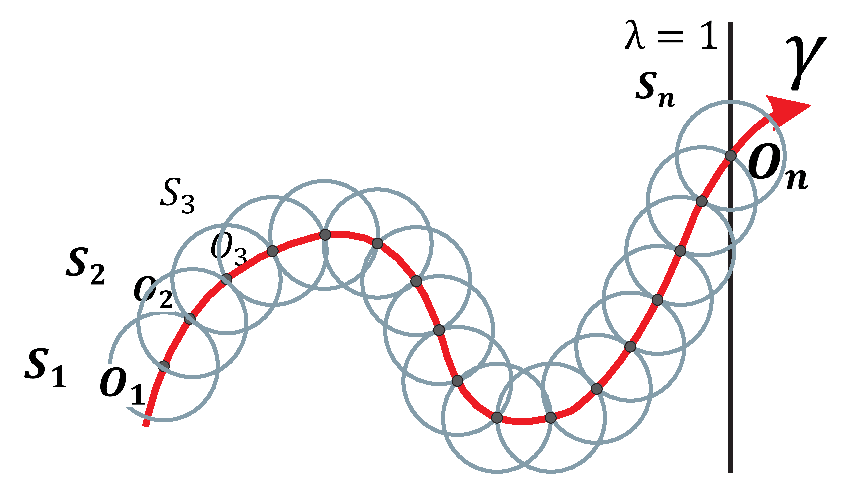
\includegraphics[width=0.2\textwidth]{imagenes/hiper2.eps} 
\caption{ Seguimiento.}
\label{fig:hiper4}
\end{center}
\end{figure}    
  
\subsection*{Predictor-Corrector Scheme}
 A proper \cite{plc1} predictor-corrector Figure \ref{fig:hiper4} scheme \cite{Hector1, Gerardo1}...
  
 
 



\section{Experiments}

The efficiency of the \cite{Park-2008} proposed...
\subsection{Successful path for maps with 200 and 2000 obstacles}

We consider two study cases...

  \vspace{-0.1 cm}
\begin{table}[H]
\begin{center}
\resizebox{9cm}{!} {
\begin{tabular}{ |c|c|c|c|c|c|c|c|c| }
\hline
\multicolumn{9}{|c|}{Environment maps}\\
\hline
\multicolumn{1}{|c}{N.Obstacles}&\multicolumn{4}{|c}{200}&\multicolumn{4}{|c|}{2000}\\
\hline
Path&1&2&3&4&1&2&3&4\\
\hline
Steps&919&898&894&999&7165&6404&7406&6953\\
\hline
Time (ms)&504&483 &504&564&41190&38840&48561&39305\\
\hline
Path length&2.10143&2.06822&2.01062&2.2497&2.59544&2.20463&2.57591&2.40284\\
\hline
\end{tabular}
}
\end{center}
\caption{Computation time and length in normalized units for two environment maps.}
\label{table:tiempos}
\end{table}

%%%jashljdhlsjahlfhsd

\section{Conclusions}
 In this work,...

\bibliographystyle{ieeetr}
\bibliography{bibliography}



\end{document}


